\chapter{Project Description}
\section{Detailed project description}
%Begin from here





\section{Beneficiaries of the project}
%Begin from here





\section{Detailed analysis}
%Begin from here
We analyze the project into following points:
\begin{enumerate}
    \item Objective:
    \begin{itemize}
        \item Apply different retrival Techniques and deal with new problems.        
        \item Deal with multimedia systems and how these systems are designed and implemented.
    \end{itemize}
    \item Concept of project:
    \begin{itemize}
        \item The basic concept of this project is how to get retrive matching data for input image or input video.        
        \item We apply this concept using some retrival techniques.
    \end{itemize}
    \item Classification of the project:
    \begin{itemize}
        \item It is a content based video/image retrival for multimedia systems.        
    \end{itemize}
    \item Project life cycle:
    \begin{itemize}
        \item Run the GUI.
        \item Insert input image or video.
        \item Select retrival technique.
        \item Get matching results if exist.        
    \end{itemize}
    \vskip 0.1in
    \item Project characteristics:
    \begin{itemize}
        \item Can deal with image and video inputs.
        \item Provide a database to store iamges and videos.
        \item Support different retrival techniques.
    \end{itemize}
\end{enumerate}        
















\section{Techniques description}
\subsection{Images techniques}

\subsubsection{Mean color}
This technique depends on computing the distance between images based on the color similarity between them. 
For RGB images the mean color of pixels is computed by finding the average color of the pixels in each channel 
separately then finding the average between the three
values that result from each channel. To get the most similar images to the input image ,the difference between the mean color the input image 
and each image in the database is computed then we apply a reasonable threshold to execlude the images with large distance.
\vskip 0.2in
Mean color is one of the most techniques used in image retreival systems 
because it can be completed without regard to image size or orientation and it needs less computational power than other techniques.


\subsubsection{Histogram}
Histogram search algorithms , characterize an image by its
color distribution or histogram. A histogram is nothing but
a graph that represents all the colors and the level of their
occurrence in an image irrespective of the type of the
image. 
\vskip 0.2in
Few basic properties about an image can be obtained
from using a Histogram. It can be used to set a threshold for
screening the images. The shape and the concentration of
the colors in the histogram will be the same for similar
objects even though they are of different colors.
\vskip 0.2in
Identifying objects in a grey scale image is the easiest one as the
histogram is almost similar as the objects have the same
colors for same objects. In order for identifying the objects
in the images or generating the histogram the system has to
obtain the array values of the frequency of occurrence of each color value -from 0 to 255- in the image.
\vskip 0.2in

\begin{figure}[H]
    \centering
    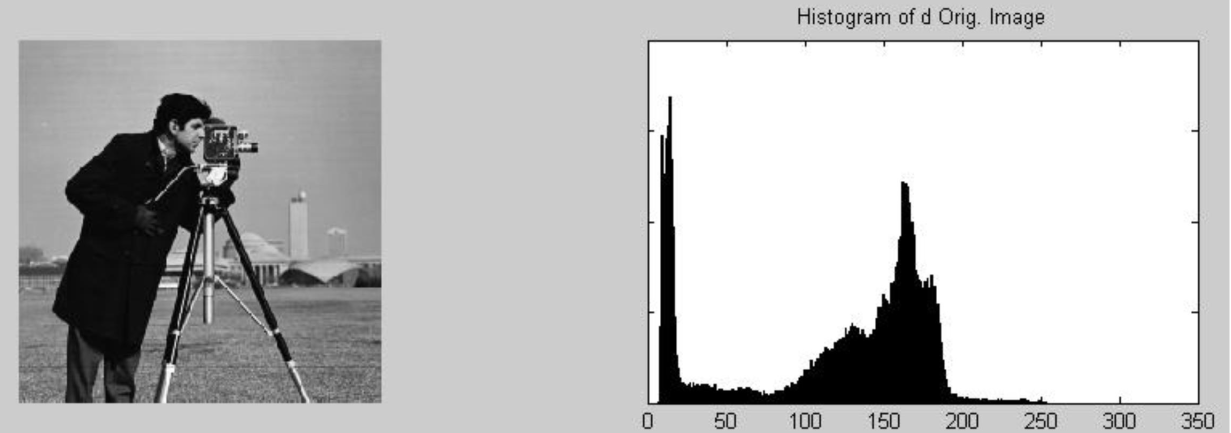
\includegraphics[width=70mm,height=40mm]{Images/hist.png}
    \caption{example for image histogram}
  \end{figure}
\vskip 0.2in

To calculate the distance between two image histogram we calculate the sum of the
smallest bin for each corresponding bins in the two histograms
for input image I and the model image M normalized to the
number of pixels in the model image.
\vskip 0.2in

\begin{figure}[H]
    \centering
    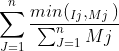
\includegraphics[width=40mm,height=20mm]{Images/eq.png}
    \caption{histogram distance equation}
  \end{figure}

  \vskip 0.2in
\subsubsection{Color Layout}
This technique is similar to histogram based technique except it solves the problem of getting results of images with a low 
histogram distance value but with a different contents.
\vskip 0.2in
In this algorithm we divide each image into 5x5 array of blocks so we get 25 sub-image then we calculate the histogram form each block.
To find the distance between to images we get the distance between the histograms of each two corresponding block, 
then we calculate the total distance by finding the summation of all blocks distance.
\vskip 0.2in

\begin{figure}[H]
    \centering
    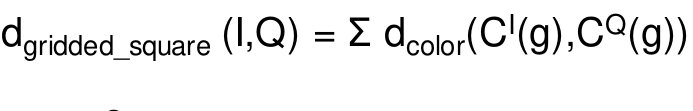
\includegraphics[width=80mm,height=20mm]{Images/cl.png}
    \caption{color layout distance equation}
  \end{figure}
  
  \vskip 0.2in

\subsection{Videos techniques}
%Begin from here
\subsubsection{Feature extraction technique}
\vskip 0.2in
To make a content based video retrieval system, we have to deal with videos as frames and compare frame with each others as images.
But applying this technique would consume a lot of memory to store the whole frame of each video.
So the key frames role appear here.
\vskip 0.2in
A key frame (or keyframe) in animation and filmmaking is a drawing or shot that defines the starting 
and ending points of any smooth transition. These are called frames because their position in time is measured in 
frames on a strip of film or on a digital video editing timeline.
\vskip 0.2in
So we make a key frame extraction operation for each video before inserting it to the database.
then we deal with key frames as the same manners of images, We caculate the histogram for each key frame and divide the range into 
five regions then we get the averge of each region resulting the five values that we store in the data base, after that we use these values
as a initial filtering to get the most similar frames of the input ,then we use the accurate -255 values- histogram to make a second step filtering.
\vskip 0.2in
\subsubsection{Distance calculation}
To get the distance between two videos we use the naive video similarity technique.
In this technique we calculate how many key frames in the query video is similar to one or more key frame in the model video, then 
we calculate the ration between these key frames to the total number of the key frames, after that we compare the distance with a threshold valueand if the 
distance is lower than this threshold, the two videos are similar otherwise they are not similar.